\documentclass[a4paper,british]{article}

% ======== General set-up

\usepackage[british]{babel} % avoids `anal-ysis', inter alia.
\usepackage[hmargin=3.5cm,vmargin=2.5cm]{geometry}
\frenchspacing
\usepackage{ifpdf} % For now, I'm just targeting pdflatex and htlatex.
\usepackage{calc} % allow infix arithmetic
\ifpdf
  \usepackage[T1]{fontenc}
  \usepackage[bitstream-charter]{mathdesign}
  \renewcommand{\sfdefault}{fvs}
\fi
\usepackage[round]{natbib}
\usepackage[utf8]{inputenc}
\usepackage{url}
\usepackage{graphicx}
\usepackage{float}
\floatstyle{ruled}
\restylefloat{figure}
\usepackage{placeins}
\usepackage{booktabs}
\usepackage{listings}
\usepackage{textcase}
\usepackage{titlesec} % to start sections on a new page
\newcommand{\sectionbreak}{\clearpage}
\usepackage{color}
\definecolor{mylinkcolour}{RGB}{0,0,160}
\usepackage{textcomp} % for \textdegree
\ifpdf
  \usepackage[unicode=true]{hyperref}
  \hypersetup{breaklinks=true,pdfborder={0 0 0},colorlinks=true,
    linkcolor=mylinkcolour,citecolor=mylinkcolour,urlcolor=mylinkcolour,
    filecolor=mylinkcolour}
\fi
%\setlength{\parindent}{0pt}
\setlength{\parskip}{4pt plus 2pt minus 1pt}
\setlength{\emergencystretch}{3em}  % prevent overfull lines
\setlength{\belowcaptionskip}{1ex}

% ======== My commands

% Custom definition list for menu items
\newcommand{\menuitemlabel}[1]{%
\mbox{\textsf{#1}}\hfil}
\newenvironment{menuitemlist}%
{\begin{list}{}{%
\renewcommand{\makelabel}{\menuitemlabel}%
\setlength{\labelwidth}{35pt}%
\setlength{\leftmargin}%
             {\labelwidth+\labelsep}}}%
{\end{list}}

\newcommand{\ppcmd}[1]{\textsf{#1}} % For `computer' text
% \newcommand{\caps}[1]{\textsc{#1}} % for acronyms and initialisms
\newcommand{\caps}[1]{\MakeTextUppercase{#1}} % for acronyms and initialisms
\newcommand{\submenu}{ \textgreater{} } % htlatex doesn't like `>'.
\newcommand{\alnifi}{$\alpha_{95}$}
\newcommand{\quot}[1]{`#1'}

% ======== Title

% automatic version number / date: see
% http://truongnotes.tumblr.com/post/13407676428/embed-mercurials-version-number-in-latex

\input hg-cmds.tex
\title{PuffinPlot User Manual}
\author{Pontus Lurcock}
\date{Version \HgVersion, \HgDate}

% ======== Document starts here.

\begin{document}

\maketitle

\tableofcontents

\section{Introduction}

This manual gives a practical guide to the usage of the PuffinPlot
palaeomagnetic data analysis program. Note that it does not elucidate the
principles of the analysis techniques themselves, and a working knowledge of
palaeomagnetic procedures is assumed. For excellent introductions to
palaeomagnetic analysis, see \cite{tauxe2010paleomagnetism} or
\cite{butler1992paleomagnetism}.

If you use PuffinPlot in the creation of published work, please cite the
PuffinPlot paper \citep{lurcock2012puffinplot}. See
Appendix~\ref{sec:citing-puffinplot} for further details.

PuffinPlot is free software, distributed under the GNU General Public
License. Please see the \ppcmd{LICENCE} file in the PuffinPlot archive
for details.

\section{Installation}

This section describes the hardware and software requirements for
running PuffinPlot, and gives instructions for installing and running
it.

\subsection{Requirements}

PuffinPlot runs on the Java platform (version 6 or later), which is
preinstalled or freely available for a variety of operating systems,
including Windows, Linux, and Mac OS X. Java is generally easy to install,
but detailed instructions for installing it are beyond the scope of this
manual; please consult the documentation for your operating system or visit
\url{http://www.java.com/} for details.

\paragraph{Java installation: Mac OS X notes.} On most versions of Mac OS X,
Java is preinstalled as standard. On version 10.7 (Lion) it must be manually
installed via \ppcmd{Applications\submenu Utilities\submenu Java
  Preferences}.

\subsection{Obtaining and installing PuffinPlot}

You may download the latest version of PuffinPlot from
\url{https://code.google.com/p/puffinplot/}. PuffinPlot is distributed as a
single zip archive file containing the program itself (in two different
variants, as detailed below) and documentation. The documentation consists of
this manual (in both HTML and PDF format) and a JavaDoc folder, containing
documentation for PuffinPlot's source code. The JavaDoc is only of interest
to users wishing to write scripts which interface directly with PuffinPlot's
internal data structures (see section~\ref{sec:scripting}).
Table~\ref{tbl:archive-contents} lists the contents of the PuffinPlot
archive. After downloading the archive, move it to the folder where you
would like PuffinPlot installed and extract its contents there.

\begin{table}[bp]
%{Fields for sample data export}
  \caption{\label{tbl:archive-contents} The contents of the PuffinPlot archive file.}
\begin{tabular}{ll} \toprule
File           & Description \\ \midrule
README         & A text file briefly describing the archive. \\
PuffinPlot.jar & The PuffinPlot program (suitable for all operating systems) \\
PuffinPlot.app & The PuffinPlot program (tailored for Mac OS X) \\
Manual         & Folder containing this manual in PDF and HTML format \\
JavaDoc        & Folder containing internal documentation for PuffinPlot \\
Example-files  & Folder containing example data files \\
LICENCE        & The licence under which PuffinPlot is distributed \\
\bottomrule
\end{tabular}
\end{table}

\subsubsection{All operating systems}

The file \textsf{PuffinPlot.jar} in the archive is the PuffinPlot program
itself, as a cross-platform jar (Java archive) file. This file is recommended
for Linux, Windows, and other non-Mac operating systems; it will also run on
Mac OS X, but the specific Mac OS X version described below is usually
preferable. The details of starting PuffinPlot vary between operating
systems, but double-clicking on the file \textsf{PuffinPlot.jar} is the most
common method. In some cases it may be necessary to right-click on the file
and select \emph{Open with Java runtime} or some similar text from a menu.
PuffinPlot can also be started from a terminal prompt by setting the current
folder to the one containing PuffinPlot, and typing \textsf{java -jar
  PuffinPlot.jar}.

\paragraph{Note for Windows users.} Under Windows, other programs may
occasionally interfere with the Java platform; if you have the Java platform
installed on Windows but are still unable to run \ppcmd{jar} files such as
\ppcmd{PuffinPlot.jar}, the situation can usually be fixed by running the
\ppcmd{jarfix} program. At the time of writing, \ppcmd{jarfix} may be
downloaded from \url{http://johann.loefflmann.net/en/software/jarfix/}.

\subsubsection{Mac OS X}

The PuffinPlot archive also contains a special variant of the program for Mac
OS X. This varient is packaged as a standard OS X application and conforms
more nearly to OS X user interface standards than the cross-platform version
described in the previous section. It is named `PuffinPlot.app', although 
the extension `.app' is usually hidden by Mac OS X.

In the extracted archive contents, the PuffinPlot application is shown as an
icon representing a puffin (specifically, the Atlantic Puffin
\emph{Fratercula arctica}). The application may then be dragged into the
Applications folder, or any other convenient place.

PuffinPlot is started by double-clicking on its application icon.

\section{Basic usage}

This section gives a brief introduction to the PuffinPlot data model and
to the features of its main window.

\subsection{A note on keyboard shortcuts}

PuffinPlot provides a large number of keyboard shortcuts for its various
capabilities; most of them involve holding down the Ctrl key while
pressing another key. On Mac OS X, these shortcuts use the command key
rather than the Ctrl key, in accordance with Apple user interface
guidelines. Throughout this manual, keyboard shortcuts will be given as
(for example) Ctrl-A. Users of Mac OS X should read these shortcuts as
command-A, etc.

\subsection{Opening a file}

To open a file, select \textsf{Open\ldots} from the \textsf{File} menu. This
will allow you to choose one or more files to open from a standard file
selection window. You may also select an entire folder; in this case
every file within the folder will be opened.

\begin{figure}[htbp]
\centering
\ifpdf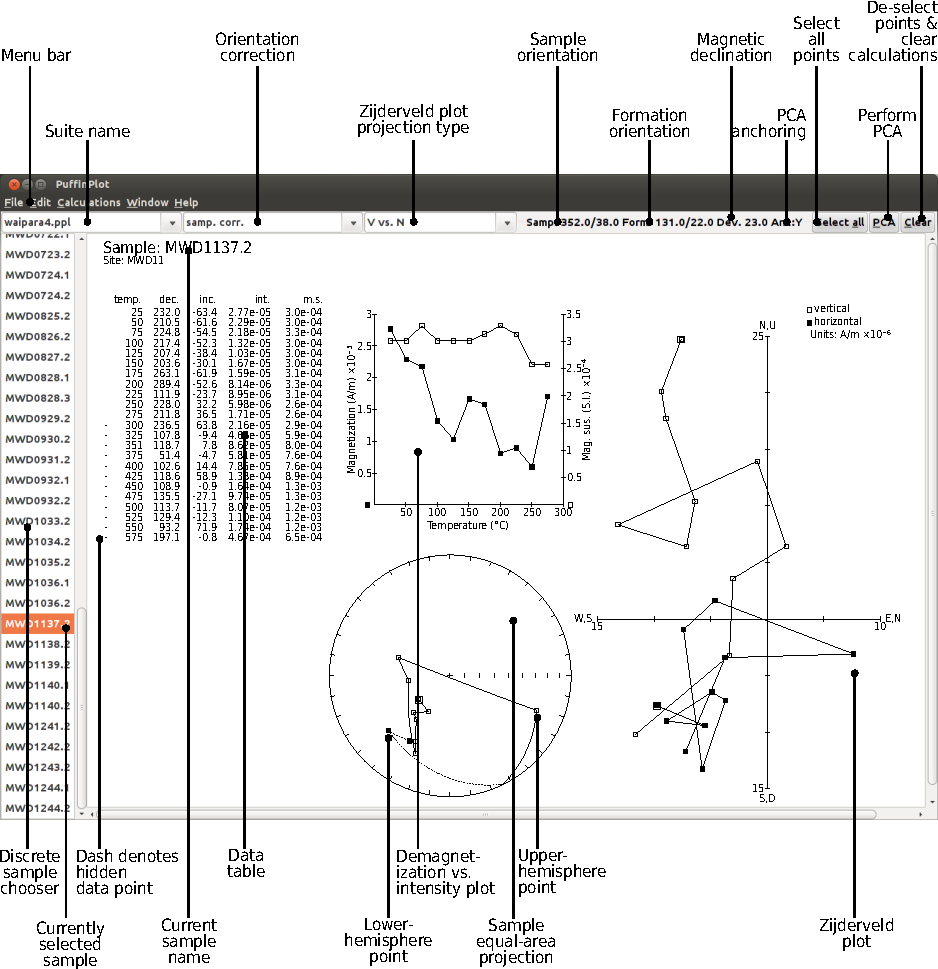
\includegraphics{figures/annot-scrnshot.pdf}
\else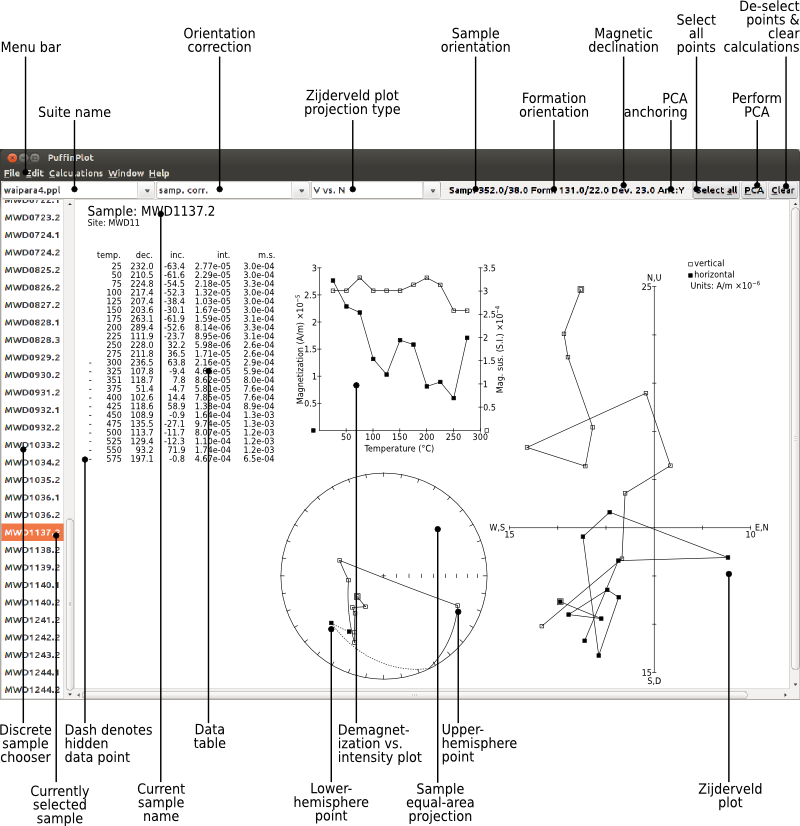
\includegraphics{figures/annot-scrnshot.png}
\fi
\caption{\label{fig:screenshot}The main window of PuffinPlot with a discrete
  file loaded, showing the default data plot layout. Data plots, information
  displays, and controls are annotated. Note that several other data plots
  are available, but are not shown by default, and that the layout may be
  freely rearranged by the user. Data points above the 275\textdegree C
  demagnetization step have been hidden.}
\end{figure}

\subsection{A tour of the main window}

Figure 1 shows an annotated screenshot of PuffinPlot's main window with
a discrete sample data file open. The bulk of the window is devoted to
the data display itself, and shows the four most popular data display
methods for palaeomagnetic data: a table, a Zijderveld plot, an
equal-area projection, and a demagnetization-intensity biplot (which
also shows an overlaid magnetic susceptibility plot). The plots are
interactive, in that individual data points may be selected by clicking
or by dragging a rectangle with the mouse.

To the left of the main plot display area is the sample chooser, which shows
a complete list of the samples within the suite, with the currently selected
sample highlighted. Multiple samples may be selected at once allowing
functions such as \caps{pca} calculation to be performed \emph{en masse}. If
a long core data file is loaded, the sample chooser is shown as a vertical
slider indicating depth rather than a list of sample names.

Above the main plot area is the toolbar, which gives convenient access
to some of the most frequently used facilities of the program. From left
to right, these are: choosers for the currently displayed data suite,
the orientation correction, and the Zijderveld projection type; displays
of the sample and formation orientations and magnetic declination; and
buttons for three of the most commonly performed actions.

At the top of the window is the menu bar, providing access to all the
program's functions in a hierarchical manner. On Mac OS, the menu bar is
at the top of the screen rather than the top of the window, and includes
an extra menu at the left, entitled \textsf{PuffinPlot}.

\subsection{Data model}

\begin{figure}[htbp]
\centering
\ifpdf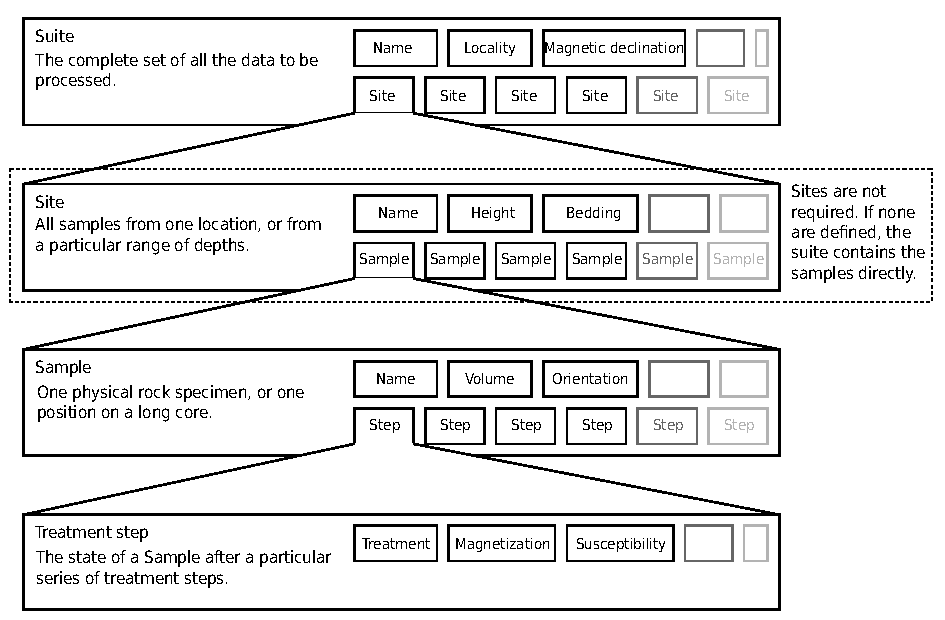
\includegraphics{figures/data-model.pdf}
\else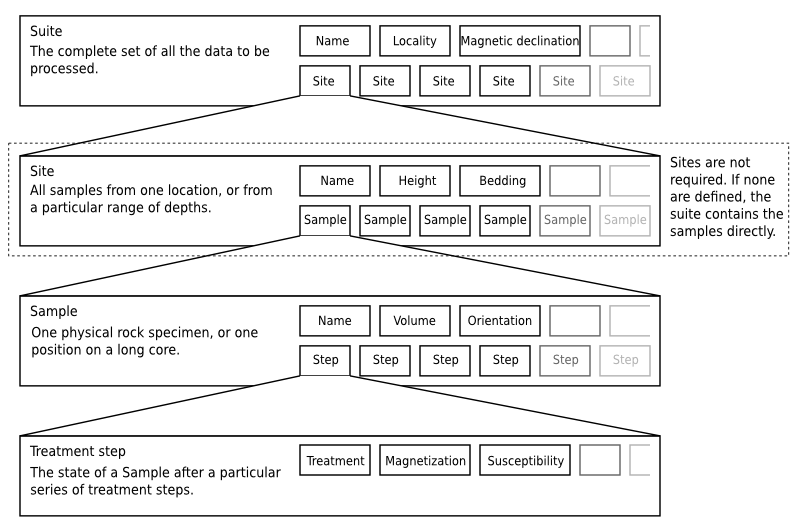
\includegraphics{figures/data-model.png}
\fi
\caption{PuffinPlot's hierarchical data model. Each layer (except the
lowest) contains multiple instances of the following layer.}
\end{figure}

PuffinPlot uses a hierarchical data structure, with higher levels containing
multiple instances of each lower level. The structure is summarized in Figure
2. At the top is the \emph{suite}, which contains all the data to be analysed
as part of a particular study. For a discrete specimen study, this will
typically correspond to a section in the field; for a long core study, it
will correspond to a core. A suite is initially created by opening one or
more data files from a magnetometer; it is saved as a file in PuffinPlot's
own format. In a discrete study, a suite contains multiple \emph{sites}. A
site corresponds to a set of samples taken from one spot in a section. A
site's associated data can include such things as bedding attitude and
stratigraphic height, as well as calculated parameters such as the mean
palaeomagnetic direction for all the samples at the site. Site are not
required: if no sites have been defined, samples are contained directly
within the suite.

Each site (or, if no sites are defined, the suite) contains multiple
\emph{samples}. A sample corresponds to a small physical volume of rock. For
a discrete study, this will usually be a typical palaeomagnetic 25mm cylinder
or IODP cube sample. For long cores, it is the portion of the core at a
particular depth. The data associated with a sample consists of information
specific to this physical unit which does not change with the application of
demagnetization techniques --- for example, a sample code or name (or, for
long cores, a depth), the field orientation of the sample, and its volume.
For discrete samples this data can also include a tensor representing
anisotropy of magnetic susceptibility, which is imported separately from an
Agico kappabridge datafile and collated with the magnetization data by
matching the sample names. The sample can also contain calculated parameters,
such as a direction fitted by principal component analysis, or a best-fitting
great circle.

Each sample contains multiple \emph{demagnetization steps}. A \emph{step}
represents a sample at a particular point during the treatment protocol. Its
associated data thus includes details of the treatment: the type (thermal,
AF, IRM, etc.) and parameters (temperature, field strength, etc.). The data
also includes the state of the sample itself --- most importantly, the
measured magnetization vector. For thermal studies, the magnetic
susceptibility is usually also recorded after every heating cycle, and is
also stored as part of the step.

\subsection{Main window features}

This section describes the parts and functions of the main PuffinPlot
window, as shown in figure~\ref{fig:screenshot}.

\subsubsection{Plot area}

The plot area is the largest part of the window, and plots the data for the
current sample using various plots. By default, four plots are shown: a
demagnetization-intensity biplot, a Zijderveld plot, an equal-area
projection, and a table of demagnetization steps. The plots can be moved and
resized (see section~\ref{sec:edit-layout}). Other plots are also
available, and the preferences window can be used to control which plots are
displayed (see section~\ref{sec:preferences}).

\subsubsection{Sample chooser}

The sample chooser sits at the leftmost edge of the main window, and
allows you to change the current sample (the one for which data is
plotted) and the set of selected samples (most of PuffinPlot's functions
operate on the currently selected samples). Often, the set of selected
samples will consist only of the current sample.

The sample chooser takes two forms, depending on whether the current
suite of data is for discrete samples or for a continuous long core
measurement.

\paragraph{Using the discrete sample chooser}

The discrete sample chooser shows the names of the samples in the current
suite. The selected sample or samples are highlighted in a different colour.
The selected sample is the current sample, and its data is displayed in the
main plot area. If more than one sample is selected, the first of the
selected samples is the current sample.

To select a single sample, click on its name. To select a contiguous range of
samples, click at one end of the range, then hold down \ppcmd{Shift} while
clicking at the other end of the range. To select multiple, non-contiguous
samples, hold down \ppcmd{Ctrl} while clicking. To select all samples, press
\ppcmd{Ctrl-A}.

\paragraph{Using the continuous sample chooser}

The continuous sample chooser is a vertical grey bar representing the total
length of the measured core, striped with horizontal white lines representing
the individual measurements at each depth. (If there are too many
measurements for all the requisite white lines to be displayed, they are
omitted.) A black triangle and line show the current depth; this is the depth
for which the data is displayed in the main window. If there are selected
samples, they are highlighted in red on the sample chooser.

To select a single depth, click on the appropriate part of the sample
chooser. To scroll rapidly through a range of samples, click and drag the
mouse along the sample chooser. To select a range of samples, hold down
\ppcmd{Shift}, then click, drag, and release the mouse on the chooser.

\paragraph{Keyboard shortcuts for sample selection}

Use \ppcmd{Ctrl-B} and \ppcmd{Ctrl-N} to change the current sample. Use
\ppcmd{Ctrl-A} to select all the samples in the current suite. You can also
use the up and down arrow keys to change the sample.

\subsubsection{\label{sec:toolbar}Toolbar}

The toolbar displays various data and provides several controls.
From left to right, these are:

\begin{description}

\item[Suite chooser.] This shows the name of the current suite of data. If
  more than one suite of data has been opened, the suite chooser allows you
  to switch between them.

\item[Orientation correction chooser.] This chooser allows you to choose
  whether data is displayed in laboratory co-ordinates (\ppcmd{uncorrected}),
  in field co-ordinates, corrected for sample orientation (\ppcmd{samp.
    corr.}), or in tectonic co-ordinates, corrected for both sample
  orientation and bedding orientation (\ppcmd{form. corr.}).

\item[Zijderveld projection type.] This chooser controls the vertical
  projection used in the Zijderveld plot. The {\em y} axis always corresponds
  to the vertical direction; the chooser controls the {\em x} axis, which may
  correspond to North (\ppcmd{V vs. N}) or East (\ppcmd{V vs. E}). The third
  option, \ppcmd{V vs. H}, projects each data point separately, in the plane
  containing itself and the origin; this is sometimes referred to as a
  `modified Zijderveld' plot.

\item[Sample orientation] (\ppcmd{Samp}). The first number is the azimuth of
  the sample orientation; the second is its either its dip angle or its hade,
  depending on the current setting in the user preferences (see
  section~\ref{sec:prefs-misc}). By default, PuffinPlot uses dip angle rather
  than hade. For a long core, the azimuth and dip will usually be 0 and 90
  respectively throughout the core.

\item[Formation orientation] (\ppcmd{Form}). The first number is either the
  azimuth of the dip for the bedding, or its strike; the second is the dip
  angle. By default PuffinPlot uses the dip azimuth rather than the strike,
  but this can be changed in the preferences window (see
  section~\ref{sec:prefs-misc}).

\item[Magnetic declination] (\ppcmd{Dev}). This is the angle between magnetic
  north and true north at the sampling site. (It is abbreviated `Dev' (for
  `deviation') to avoid any possible confusion with the declinations of
  sample magnetizations.)

\item[Select all] selects all the points in the current sample.

\item[\caps{Pca}] performs principal component analysis for the selected
  points of all the selected samples.

\item[Clear calculations] de-selects all the points in all the selected
  samples, and clears the results of any calculations done on them, such as
  \caps{pca} or great-circle analysis.

\end{description}

\section{Detailed usage}

This section gives a methodical account of PuffinPlot's features.

\subsection{Catalogue of functions}

This section lists all the items in PuffinPlot's menus, giving a brief
description of the functionality associated with each one.

\subsubsection{\label{sec:menu-file}File menu}

This menu contains functions connected with opening, closing, and
saving files.

\begin{menuitemlist}

\item[File\submenu Open\ldots] loads one or more files of demagnetization
  data into PuffinPlot as a new suite. See
  section~\ref{sec:file-types} for details of supported filetypes.

\item[File\submenu Import data\ldots] imports data from a file format
  specified by the user. This feature allows most textual, tabular data files
  to be read by PuffinPlot. See section~\ref{sec:import-data} for details.

\item[File\submenu Open recent file] is a submenu which contains the names of
  the last eight files which have been opened in PuffinPlot, allowing them to
  be opened again with a single click.

\item[File\submenu Save] saves the current suite as a PuffinPlot file. If
the suite was opened from a PuffinPlot file or if it has been previously
saved as a PuffinPlot file, it will immediately be saved to that file. If no %
PuffinPlot file is associated with this suite yet, a standard ‘save file’
dialog box will prompt you for a file name and location.

\item[File\submenu Save as\ldots] allows you to save the current suite to a
different filename or location.

\item[File\submenu Close] closes the current suite, removing it from
PuffinPlot's data display.

\item[File\submenu Export data] is a submenu allowing the export of
various kinds of data to \caps{csv} files.

\item[File\submenu Export data\submenu Export sample calculations\ldots]
  saves a file containing all the data associated with individual samples.
  Table~\ref{tbl:export-sample} describes the fields which make up the file.

\begin{table}[tp]
%{Fields for sample data export}
  \caption{\label{tbl:export-sample} List of fields in exported sample data file, Note that, in addition to the predefined fields, any custom user annotations (see section~\ref{sec:annotations}) will also be exported in this file.}
\begin{tabular}{lp{90mm}} \toprule
Field name           & Description \\ \midrule
Suite                & Suite name \\
sample               & Sample name \\
\caps{nrm} intensity (A/m) & \caps{Nrm} intensity in A/m \\
\caps{ms} jump temp. (\textdegree C) & For thermal demagnetization, the
temperature step at which the first jump in magnetic susceptibility occurs.
A jump is defined as a susceptibility of at least 2.5 times the previous value.
\\
\caps{pca} dec. (\textdegree)     & Declination of \caps{pca} direction (\textdegree)\\
\caps{pca} inc. (\textdegree)     & Inclination of \caps{pca} direction (\textdegree)\\
\caps{pca} \caps{mad}1 &  The Maximum Angle of Deviation
for the planar \caps{pca} fit; the smaller the value, the more coplanar the points. See section~\ref{sec:plot-types} for more details.\\
\caps{pca} \caps{mad}3 & The Maximum Angle of Deviation
for the linear \caps{pca} fit; the smaller the value, the more collinear the points. See section~\ref{sec:plot-types} for more details.\\
\caps{pca} anchored    & `Y' if the \caps{pca} fit was anchored; `N' if not \\
\caps{pca} equation    & The Cartesian equation of the \caps{pca} best-fit line \\
\caps{pca} start (\textdegree C or mT)      & Field (in mT) or temperature 
(in \textdegree C) of first demagnetization step used for \caps{pca} analysis\\
\caps{pca} end (\textdegree C or mT)        & Field (in mT) or temperature 
(in \textdegree C) of last demagnetization step used for \caps{pca} analysis \\
\caps{pca} contiguous       & `Y' if
all steps between the first and last were selected for \caps{pca};
`N' if any were omitted \\
\caps{GC} dec (\textdegree) & the declination of the pole to the fitted great circle, if any \\
\caps{GC} inc (\textdegree) & the inclination of the pole to the fitted great circle, if any \\
\caps{GC} strike (\textdegree) & the strike of the plane of the fitted great circle, if any \\
\caps{GC} dip (\textdegree) & the dip of the plane of the fitted great circle, if any \\
\caps{GC} \caps{mad}1 & the \caps{mad}1 value for the great circle fit,
indicating goodness of fit (smaller is better). See section~\ref{sec:plot-types} for more details. \\
\caps{GC} npoints & the number of points used for the great-circle fit \\
\caps{mdf} half-intensity (A/m)  & half of the \caps{nrm} (in A/m) \\
\caps{mdf} demagnetization (\textdegree C or mT) & the demagnetization treatment level
at which the \caps{nrm} was reduced to half (in \textdegree C or mT) \\
\caps{mdf} midpoint reached & `Y' if magnetization
intensity reached half the \caps{nrm} intensity during demagnetization;
`N' otherwise \\
\caps{ams} dec1 & declination of major axis of \caps{ams} tensor \\
\caps{ams} inc1 & inclination of major axis of \caps{ams} tensor \\
\caps{ams} dec2 & declination of intermediate axis of \caps{ams} tensor \\
\caps{ams} inc2 & inclination of intermediate axis of \caps{ams} tensor \\
\caps{ams} dec3 & declination of minor axis of \caps{ams} tensor \\
\caps{ams} inc3 & inclination of minor axis of \caps{ams} tensor \\
{\em [annotations]}  & Any user-defined annotations
are also exported as part of the sample export file. See
section~\ref{sec:annotations} for details. \\ \bottomrule
\end{tabular}
\end{table}

\item[File\submenu Export data\submenu Export site calculations\ldots] saves
  a file containing (for suites with discrete samples) all the data
  associated with sites. Table~\ref{tbl:export-site} describes the fields
  which make up this file.

\begin{table}[tp]

  \caption{\label{tbl:export-site} List of fields in exported site data file}

\begin{tabular}{lp{90mm}} \toprule
  Field name      & Description \\ \midrule
  site            & Name of site \\
  Fisher dec.     & Mean declination of \caps{pca} directions (\textdegree) \\
  Fisher inc.     & Mean inclination of \caps{pca} directions (\textdegree) \\
  Fisher a95      & \alnifi{} of mean \caps{pca} direction (\textdegree) \\
  Fisher k        & {\em k}-value of mean \caps{pca} direction \\
  \caps{gc} valid & `Y' if the great-circle fit
  is valid, `N' otherwise. See section~\ref{sec:prefs-misc} for
  details on the validity test and how it may be customized. \\
  \caps{gc} dec. (°) & Declination of great-circle direction (\textdegree) \\
  \caps{gc} inc. (°) & Inclination of great-circle direction (\textdegree) \\
  \caps{gc} a95 (°) & \alnifi{} for great-circle direction (\textdegree) \\
  \caps{gc} k     & {\em k}-value for great-circle direction \\
  \caps{gc n}     & Number of great circles used in great-circle fit \\
  \caps{gc m}     & Number of \caps{pca} directions used in great-circle fit \\
  \caps{gc} min points & the smallest number of points used to define
    any of the great circles fitted at this site \\
  \caps{t}1min & See note below \\
  \caps{t}1max & See note below \\
  \caps{t}2min & See note below \\
  \caps{t}2max & See note below \\ \bottomrule
\end{tabular}

\smallskip

Note on \caps{t}1min, \caps{t}1max, \caps{t}2min, and \caps{t}2max: these
four parameters give the ranges of demagnetization steps used to fit the
circles. \caps{t}1 denotes the first (lowest) demagnetization step in a
circle path for an individual sample, and \caps{t}2 the last (highest).
\caps{t}1min is the minimum of the \caps{t}1 values across all the circles
for the site, and \caps{t}1max the maximum. Similarly, \caps{t}2 denotes the
last step used in a single circle, and \caps{t}2min--\caps{t}2max is the
range of its values across all the samples at a site.

\hrulefill

\end{table}

\item[File\submenu Export data\submenu Export suite calculations\ldots] saves
  a \caps{csv} file containing the Fisherian parameters for mean directions
  calculated across the entire suite; see the documentation for the
  \ppcmd{Calculate\submenu Suite means} menu item
  (section~\ref{sec:functions-calcs}) or details.

\item[File\submenu Export data\submenu Export multi-suite calculations\ldots]
  saves a \caps{csv} file containing the Fisherian parameters for mean
  directions calculated across all the currently open suites; see the
  documentation for the \ppcmd{Calculate\submenu Multi-suite means} menu item
  (section~\ref{sec:functions-calcs}) or details.

\item[File\submenu Export data\submenu Export IRM data\ldots] saves files
  containing \caps{irm} acquisition data. It produces a folder of files, one
  for each sample in the suite. Each file is in tab-delimited text format,
  and each line within the file contains the \caps{irm} field strength and
  the magnetization intensity of the sample after application of that field.

\item[File\submenu Export graphics] is a submenu with various options
  for exporting the plots for the current and selected samples.
  See section~\ref{sec:graphics-export} for full details.

\item[File\submenu Page Setup\ldots] opens a window allowing you
to change the paper size, orientation, and margins for printing.

\item[File\submenu Print\ldots] opens a window allowing you to print the
  selected samples. Note that {\em only} the selected samples will be
  printed, so if you wish to print the whole suite use \ppcmd{Edit\submenu
    Select all} first. On most systems this will also allow you to print to a
  \caps{pdf} file; Windows users may need to install a virtual \caps{pdf}
  printer, such as Cute\caps{pdf} Writer or Bullzip \caps{pdf} Printer, in
  order to produce \caps{pdf} files.

\item[File\submenu Print suite EA window\ldots] prints the contents of a
  separate window showing an equal-are plot of sample/site directions through
  the suite; see section~\ref{sec:menu-window} for more details.

\item[File\submenu Print site EA window\ldots] prints the contents of a
  separate window showing an equal-area plot of directions at the current
  site; see section~\ref{sec:menu-window} for more details.

\item[File\submenu Import AMS\ldots] imports \caps{ams} data from a file. The
  file must be in the \caps{.asc} format produced by the \ppcmd{Safyr}
  program distributed with \caps{Agico} kappabridges. The \caps{ams} data is
  assigned to the appropriate samples within the suite by matching the sample
  names specified in the \caps{asc} file with the sample names for the
  demagnetization data. If the \caps{ams} file contains data for samples not
  in the suite, these samples will be created and added to the suite.
  \caps{Ams} data is not displayed by default; the equal-area plot of
  \caps{ams} data can be activated from the \ppcmd{Preferences} window.

\item[File\submenu Run Python script\ldots] runs a user-specified
  external script written in the Python programming language.
  See section~\ref{sec:scripting} for details.

\item[File\submenu Export preferences\ldots] saves your current preferences
  to a file. In conjunction with the \ppcmd{Import preferences} feature, this
  allows you to transfer your preferences from one computer to another. It
  also allows you to keep multiple sets of preferences and switch between
  them as needed. Probably the most useful application is to save different
  plot layouts for different sets of data.

\item[File\submenu Import preferences\ldots] sets your preferences from a
  file saved using \ppcmd{Export preferences}. See the description of
  \ppcmd{Export preferences} for details.

\item[File\submenu Clear preferences] clears all changed preferences,
  resetting them to their default values.

\item[File\submenu Preferences\ldots] opens the preferences window. See
  section~\ref{sec:preferences} for details. On Mac OS X, this item is found
  on the \ppcmd{PuffinPlot} menu to the left of the \ppcmd{File} menu, rather
  than on the \ppcmd{File} menu.

\item[File\submenu Quit] terminates PuffinPlot. On Mac OS X, this item is
  found on the \ppcmd{PuffinPlot} menu to the left of the \ppcmd{File} menu,
  rather than on the \ppcmd{File} menu.

\end{menuitemlist}

%\FloatBarrier
\subsubsection{Edit menu}

The \ppcmd{Edit} menu provides various basic functions mainly
to do with manipulation of data points.

\begin{menuitemlist}

\item[Edit\submenu Select all] selects all the points in all the selected
  samples, excluding points which have been hidden (see \ppcmd{Hide points}
  below).

\item[Edit\submenu Clear selection] de-selects all the points in all the
  selected samples.

\item[Edit\submenu Edit layout] allows you to reposition and resize the plots
  in the main display area. See section~\ref{sec:edit-layout} for details.

\item[Edit\submenu Reset layout] resets the sizes and positions of all the
  plots to their default values.

\item[Edit\submenu Corrections\ldots] opens a window which allows you to
  change the sample orientation, formation orientation, and local magnetic
  declination for all the selected samples. Each correction type can be
  individually changed without affecting the values of the others. For
  convenience, sample orientation can be specified using either dip angle or
  hade; it is possible but pointless to enter values for both of these
  parameters, since one will overwrite the other. Similarly, formation
  orientation can be specified using either dip azimuth or strike.

\item[Edit\submenu Set treatment type\ldots] opens a window which allows you
  to change the treatment type for the selected samples. Normally, the
  treatment type will be automatically determined on opening a data file. If
  the file does not specify the treatment type, PuffinPlot will attempt to
  guess it. \ppcmd{Set treatment type} allows you to set the treatment type
  explicitly in cases where PuffinPlot guesses wrong, or where the wrong
  treatment type is given in the data file.

\item[Edit\submenu Copy point selection] copies the selected treatment steps
  for the current sample to an invisible `clipboard'. The selection can be
  pasted from the clipboard to other samples (see \ppcmd{Paste point
    selection}), selecting the same demagnetization steps in those samples.
  This is useful for selecting the same treatment steps in a large number of
  samples without having to manually select them for each sample.

\item[Edit\submenu Paste point selection] takes the selected treatment steps
  from the clipboard (see \ppcmd{Copy point selection}) and selects the same
  treatment steps in all the selected samples.

\item[Edit\submenu Flip selected samples] is a submenu allowing the selected
  samples to be rotated 180\textdegree{} around a selected axis. Such
  functionality is rarely required but can be useful, for example, when it is
  found that a sample has been incorrectly oriented during measurement, or
  when converting between different orientation conventions.

\item[Edit\submenu Flip selected samples\submenu Flip samples around X axis]
  rotates the magnetic moment values for all selected samples
  180\textdegree{} around the X axis.

\item[Edit\submenu Flip selected samples\submenu Flip samples around Y axis]
  rotates the magnetic moment values for all selected samples
  180\textdegree{} around the Y axis.

\item[Edit\submenu Flip selected samples\submenu Flip samples around Z axis]
  rotates the magnetic moment values for all selected samples
  180\textdegree{} around the Z axis.

\item[Edit\submenu Edit sites] is a submenu allowing site names to be
  set for samples in various ways.

\item[Edit\submenu Edit sites\submenu Set site name\ldots] allows a single
  site name to be set for all the selected samples.

\item[Edit\submenu Edit sites\submenu Set sites from sample names\ldots] sets
  site names for the selected samples by taking specified characters from the
  sample names. The characters to use are specified by a list of
  comma-separated numbers and number ranges; for example, entering
  \ppcmd{1,3,5-8} would give each selected sample a site name composed of the
  first, third, and fifth to eighth characters of the sample name, so that
  a sample with the name \ppcmd{FFQB0529.1} would get the site name
  \ppcmd{FQ0529}. The table below gives some further examples.

\begin{tabular}{lll} \toprule
Sample name & Character selection & Resulting site name \\ \midrule
FFQB0529.1 & 1,3,5-8 & FQ0529 \\
FFQB0529.1 & 4-6 & B05 \\
CiLpA-10-53 & 1-2,5,7-8 & CiA10 \\
CiLpA-10-53 & 3-4,9-11 & Lp-53 \\
\bottomrule \end{tabular}

\item[Edit\submenu Edit sites\submenu Set sites by depth\ldots] sets site
  names in continuous suites using the depths of the individual samples.
  PuffinPlot asks for a thickness value, and groups the samples within the
  core into sites of that thickness, effectively `slicing' the core into
  equally thick sites. Each site is named after the shallowest depth within
  it.

\item[Edit\submenu Hide points] hides all the selected points in all the
  selected samples. This removes them from all the graphical plots (which
  will be rescaled to avoid unnecessary blank space), but not from the data
  table in the main plot window; on the data table, hidden data points are
  marked with a dash symbol (--) to their left. Hidden points can be restored
  using the \ppcmd{Show all points} menu item.

\item[Edit\submenu Show all points] restores all hidden points in all the
  selected samples.

\item[Edit\submenu Edit custom flags\ldots] allows you to add or remove
  user-defined flags for the suite; see section~\ref{sec:annotations} for
  details.

\item[Edit\submenu Edit custom notes\ldots] allows you to add or remove
  user-defined note categories for the suite; see
  section~\ref{sec:annotations} for details.

\item[Edit\submenu Rescale mag. sus.\ldots] scales all the magnetic
  susceptibility values for the suite by a specified factor. This is useful
  since magnetic susceptibility meters typically do not report values in
  standard S.I. units. Note that, unlike many PuffinPlot operations, the
  scaling is applied to the {\em entire suite}, not just the selected
  samples.

\end{menuitemlist}

\subsubsection{\label{sec:functions-calcs}Calculations menu}

The calculations menu provides facilities for calculating magnetic
parameters and directions. Note that most calculations operate on
all the selected samples, not just the current sample.

\begin{menuitemlist}

\item[Calculations\submenu Calculate \caps{pca}] calculates a best-fitting
  line to all the selected points in all the selected samples, using
  principal component analysis \citep{kirschvink1980least}. The \caps{pca}
  direction is projected onto the Zijderveld plot. If the `\caps{pca}
  anchored' menu item (below) is ticked, the resulting \caps{pca} fit line
  will be anchored to the origin; if `\caps{pca} anchored' is not ticked, the
  \caps{pca} fit will be unanchored.

\item[Calculations\submenu \caps{pca} anchored] is a menu item which may be
  toggled on or off. When it is on, a tick mark appears next to it, and
  \caps{pca} analyses are constrained to pass through the origin. In general,
  it is appropriate to anchor the \caps{pca} if the analysed points are known
  to represent the final demagnetization component -- that is, they are
  trending directly towards the origin, and deviations from this path are
  known to be due to measurement noise rather than an offset in the true
  magnetization vectors. Leaving \caps{pca} unanchored allows analysis of a
  non-final component, provided that it is sufficiently well separated from
  other components.

\item[Calculations\submenu Fisher by site] calculates a Fisherian mean
  direction for each selected site using the \caps{pca} directions of its
  samples.

\item[Calculations\submenu Suite means] calculates Fisherian means across all
  the selected samples, and opens a new window showing an equal-area plot of
  the \caps{pca} directions, the mean direction, and the 95\% confidence
  circle. Two sets of means are actually calculated: one set is calculated
  from the \caps{pca} directions of individual samples, and the other from
  the site mean directions (if any have been computed). Note that, if there
  are site means computed by great-circle intersection, only those considered
  valid are used; see section~\ref{sec:prefs-misc} for details of the
  validity test. Each set of means consists of an overall mean and individual
  means for the upper and lower hemisphere, to cater for data sets containing
  reversals. All these means can be exported as a \caps{csv} file using the
  \ppcmd{File\submenu Export Data\submenu Export suite calculations\ldots}
  menu item. Note that (like most PuffinPlot functions) this feature operates
  on all the \emph{selected} samples; to calculate means for the entire suite
  you must first select all the samples.

\item[Calculations\submenu MDF] calculates the Median Destructive Field (or,
  for thermal demagnetization, the Median Destructive Temperature) of the
  selected samples. This is the field (or temperature) at which the intensity
  of the sample's remanence has been reduced to half of its initial value.
  Once calculated, it is displayed on the demagnetization-intensity plot, and
  can be saved as part of the exported sample data.

\item[Calculations\submenu Clear sample calculations] de-selects all the
  points in all the selected samples, and clears the results of any
  calculations done on them, such as \caps{pca} or great-circle analysis.

\item[Calculations\submenu Fit great circle] calculates and displays a
  best-fitting great circle for all the selected points in all the selected
  samples.

\item[Calculations\submenu Great circles] calculates a best-fitting direction
  for all the great circles fitted at the current site, using the algorithm
  of \cite{mcfadden1988circles}. The great-circle fit is shown both in the
  \ppcmd{Equal-area (site)} plot in the main window (if the plot has been
  activated in the preferences), and in a separate window which is opened
  automatically.

\item[Calculations\submenu Clear site calculations] clears the
results of any calculations associated with the selected {\em sites}
(as opposed to samples); at present, this amounts to clearing the
best-fit great-circle direction for each selected site.

\item[Calculations\submenu Multi-suite means] calculates Fisherian means
  across all the samples in \emph{all} the currently opened suites. the
  results are not plotted, but they are shown in a pop-up window and can be
  saved using the \ppcmd{File\submenu Export data\submenu Export multi-suite
    calculations\ldots} menu item.

\end{menuitemlist}

\paragraph{\caps{Ams} calculations}

PuffinPlot can show the results of statistical calculations on \caps{ams}
tensors, giving mean directions and confidence ellipses for the principal
axes by one of three methods; at present, however, these calculations cannot
be performed by PuffinPlot itself. Instead, it makes use of two Python
scripts from the PmagPy suite \citep{tauxe2010paleomagnetism},
\ppcmd{bootams.py} and \ppcmd{s\_hext.py}. In order to calculate \caps{ams}
statistics, these scripts must first be installed on the computer running
PuffinPlot, and the folder containing them must be specified in the
\ppcmd{Preferences} window. The PmagPy programs may be obtained from
\url{http://earthref.org/PMagPy/}.

All \caps{ams} calculations operate on the currently selected samples.
\cite{tauxe1998directions} and chapter 13 of \cite{tauxe2010paleomagnetism}
give more details of tensor statistics, particularly with regard to the
application of bootstrap methods.

\begin{menuitemlist}

\item[Calculations\submenu Calculate bootstrap \caps{ams}] calculates
bootstrap statistics using the \ppcmd{bootams.py} program, producing
Kent error ellipses which are shown on the \caps{ams} plot in the main
window.

\item[Calculations\submenu Parametric bootstrap \caps{ams}] calculates
bootstrap statistics using the \ppcmd{bootams.py} program, producing Kent
error ellipses which are shown on the \caps{ams} plot. It differs from the
previous function in employing a parametric bootstrap, which can provide more
realistic confidence intervals for small numbers of samples on the (often
reasonable) assumption that measurement uncertainties are normally
distributed across the selected samples.

\item[Calculations\submenu Calculate Hext on \caps{ams}] calculates
\cite{hext1963tensors} statistics using the \ppcmd{s\_hext.py} program
and displays the mean directions and error ellipses on the \caps{ams} plot.

\item[Calculations\submenu Clear \caps{ams} calculations] Clears
any previously done bootstrap and Hext calculations.

\end{menuitemlist}

\subsubsection{\label{sec:menu-window}Window menu}

This menu allows you to open or close auxiliary windows.

\begin{menuitemlist}

\item[Window\submenu Data table] opens (or closes) a window showing
all the demagnetization data for the current sample as a table. This
table is far more extensive than the brief table displayed in the
main window, and allows data to be selected and copied to the clipboard
so that it can be pasted into a spreadsheet or text editor.

\item[Window\submenu Site equal-area plot] opens (or closes) a window
  containing an equal-area plot for the current site; the plot is created by
  selecting the \ppcmd{Calculations\submenu Fisher by site} or
  \ppcmd{Calculations\submenu Great circles} menu items, and may be printed
  using the \ppcmd{File\submenu Print site EA window\ldots} menu item. Note
  that the main display area provides a similar plot; this window can be
  useful for a quick inspection of site data at a larger scale without
  editing the main plot layout.

\item[Window\submenu Suite equal-area plot] opens (or closes) a window
  containing an equal-area plot of sample or site directions across the whole
  suite; the plot is created by selecting the \ppcmd{Calculations\submenu
    Suite means} menu item, and may be printed using the
  \ppcmd{File\submenu Print suite EA window\ldots} menu item. Note that the
  main display area provides a similar plot; this window can be useful for a
  quick inspection of suite data at a larger scale without editing the main
  plot layout.

\end{menuitemlist}

\subsubsection{Help menu}

\begin{menuitemlist}

\item[Help\submenu PuffinPlot website] opens the PuffinPlot website 
using the default web browser.

\item[Help\submenu Cite PuffinPlot\ldots] opens a window containing
information on the PuffinPlot paper \citep{lurcock2012puffinplot}
and how to cite it.

\item[Help\submenu About PuffinPlot] displays some brief information
about PuffinPlot, including the version. On Mac OS X, this item is
also present on the \ppcmd{PuffinPlot} menu.

\end{menuitemlist}

\subsection{Features}

This section presents PuffinPlot's features in moderate detail.

\subsubsection{\label{sec:file-types}Supported file types}

PuffinPlot can automatically open four types of file: its own filetype
(filename suffix \ppcmd{ppl}); data produced from 2\caps{g} cryomagnetometers
(filename suffix \ppcmd{dat}); data in the Caltech format (\ppcmd{sam}, with
associated data files in same folder); and data from the {\sf Zplot} program
by Stephen Hurst (filename suffix \ppcmd{txt}). Note that there are different
ways to read 2\caps{g} data files: users are encouraged to read
section~\ref{sec:prefs-2g-import} and ensure that the preferences are
correctly set for their needs.

In general, support for other file formats is straighforward to add, and most
tabular textual file formats can be opened using the \ppcmd{File\submenu
  Import data\ldots} function.

\subsubsection{\label{sec:import-data}Importing data}

When \ppcmd{File\submenu Import data\ldots} is selected, PuffinPlot shows a
window allowing you to describe a text-based, tabular file format; once you
have specified a format, you can choose one or more files in that format,
which PuffinPlot will then open. The file is assumed to contain one magnetic
measurement per line. The file format specification consists of several
parts, which are described below.

\paragraph{General settings} describes parameters relating to the file as a
whole, rather than individual columns.

\begin{description}

\item[Number of header lines to skip] Data files may include extra data
  (`header lines') at the start of the file, most often a line containing
  textual descriptions of the columns. This field lets you specify how many
  lines PuffinPlot should ignore at the start of the file, letting it
  skip over them.

\item[Measurement type] This specifies whether the files contain discrete
  or long core measurements.

\item[Treatment type] This specifies the type of treatment applied to
  the samples -- thermal, AF, IRM, etc.

\item[Column separator] For files which do not use fixed-width columns (for
  example, CSV files), this drop-down lets you select the character used
  to separate the columns. If `Use fixed-width columns' is selected, the
  column separator is not used.

\item[Use fixed-width columns] Tabular text files usually use one of two
  conventions for separating columns: either the columns have widths which
  differ from line to line, and are separated with a special character such
  as a comma or tab; or the columns have the same width in every line, and
  are padded out to this width with space characters when the contents are
  shorter than the column width. Select this tick box to specify that the
  file format has fixed-width columns. In this case, the column separator will
  be ignored and you must specify the widths of the columns (see below).
  If this box is not selected, the column widths are ignored.

\item[Column widths] If your file format uses fixed-width columns, you must
  specify them here as a list of numbers separated by commas. For example, if
  you have six columns, with the first being ten characters wide and the rest
  eight characters wide, you would enter 10,8,8,8,8,8 in this box. If your
  file format does not use fixed-width columns, this box is ignored.

\end{description}

\paragraph{Column definitions}

\begin{description}

\item[Column no.] This is the number of the column to read; columns are
  numbered from left to right, starting at 1.

\item[Column contents] This is the data to read from the specified column.
  Note that not all data types need to be specified for a file format; at
  minimum, it is sufficient to specify the demagnetization step the three
  components of the magnetization vector (either as X, Y, and Z moments, or
  as declination, inclination, and magnetization).

\end{description}

\subsubsection{Selecting points}

For most of PuffinPlot's functions, the data points of interest must be
selected before anything can be done to them. You can select data points
simply by clicking on them; if you click on a selected point it will be
de-selected. Selected points are drawn in red to distinguish them from the
black unselected points. Note that the notional data point itself is the
thing being selected, not the visual representation that you click on. Thus,
if you click on a point in one plot, the corresponding point in all the
visible plots will also turn red, since they are visual representations of
the same datum.

Since data points are relatively small, clicking accurately on them can be
inconvenient. PuffinPlot offers two alternative selection methods to
alleviate this problem. Firstly, by holding down the \ppcmd{Shift} key, you
can select a point simply by left-clicking near it; holding \ppcmd{Shift} and
right-clicking will de-select nearby points instead. Secondly, you can
left-click, hold the button, and drag the pointer across the graph, creating
a rectangle. Every point within the rectangle will be selected. Dragging a
rectangle with the right button will instead de-select every point within the
rectangle.

\subsubsection{Working with multiple samples}

Since most PuffinPlot operations are automatically applied to all the
selected samples, repetitive analysis work can often be done automatically
using the \ppcmd{Copy point selection} feature. For example, if you wish to
apply a \caps{pca} to the 100--250\textdegree{}C demagnetization range of a
series of 50 samples, it can be done in four quick steps:

\begin{enumerate}

\item For the first sample, select the points corresponding to the
  100--250\textdegree{}C demagnetization range.

\item Select the 50 samples using the sample chooser, keeping the
  first sample as the current one.

\item Use \ppcmd{Copy point selection} on the \ppcmd{Edit} menu
  (or press \ppcmd{Ctrl-Shift-C} to select the corresponding points
  in all the selected samples.

\item Select \ppcmd{\caps{pca}} from the \ppcmd{Calculations} menu,
  or press \ppcmd{Ctrl-R}.

\end{enumerate}

This will immediately perform \caps{pca} on all 50 selected samples.

\subsection{Plots and other data displays}

\subsubsection{\label{sec:plot-types}Available plot types}

This section lists and briefly describes the available plot types in
PuffinPlot. Some of them are not displayed by default, but these may be
activated via the preferences window (see section~\ref{sec:preferences}).
Note that the term `plot' is used rather loosely in this manual to refer to
any movable element displaying data within the main window. Thus, the `plots'
listed below include textual elements such as legends and tables.

\begin{menuitemlist}

\item[Equal-area (sample)] is a Lambert azimuthal equal-area projection
  showing the directions of the current sample's magnetization vectors.
  Successive points are connected by great-circle segments. Points in the
  upper hemisphere are shown as unfilled (white) and connected by solid
  lines; points in the lower hemisphere are filled (black) and connected by
  dashed lines. If a great circle fit has been calculated for the sample, it
  is shown on this plot, and the pole to the great circle is shown as a
  triangle.

\item[Zplot] is a Zijderveld plot, overlaying an orthographic projection in
  the horizontal plane with an orthographic projection in a chosen vertical
  plane. The vertical plane can be controlled using the chooser on the
  toolbar; see section~\ref{sec:toolbar} for details. The horizontal
  projection is shown with filled points, and the vertical projection with
  unfilled points. If a \caps{pca} fit has been calculated for this sample,
  the two projections of the \caps{pca} lines are overlaid on the plot in
  blue. (If the \ppcmd{V vs. H} vertical projection is selected, only the
  horizontal projection of the \caps{pca} line is shown, since \ppcmd{V vs.
    H} effectively uses a different vertical projection for each point.) The
  appearance of the \caps{pca} lines can be changed using the Preferences dialog
  (see section~\ref{sec:prefs-misc}).

\item[Demag.] is a plot of demagnetization step (in mT or \textdegree C)
  versus intensity of magnetization (in A/m), shown as a line of filled
  points. If magnetic susceptibility measurements have been taken, they are
  overlaid on the same plot as unfilled points, with the scale shown on the
  right of the graph.

\item[Data table] is a table in which each row represents one demagnetization
  step for the current sample. The columns, from left to right, give the
  demagnetization step, declination, inclination, intensity, and magnetic
  susceptibility. Selected points are denoted by an asterisk (*) to their
  left; hidden points are denoted by a dash (--) to their left.

\item[Sample parameters] shows the results of \caps{pca} and/or great-circle
  fits for data in the current sample. If neither of these calculations has
  been done, this plot is invisible. When visible, it shows the inclination
  and declination of the first principal component, which corresponds to a
  least-squares linear fit. It also shows the maximum angular deviation
  (\caps{mad}) values \caps{mad}1 and \caps{mad}3, which function as
  goodness-of-fit parameters (smaller is better). The \caps{mad}1 value gives
  an indication of how nearly the points lie in a single plane; the
  \caps{mad}3 value gives an indication of how nearly they lie along a single
  line. \caps{Pca} analysis and \caps{mad} values are explained in
  \cite{kirschvink1980least} and in section 9.7 of
  \cite{tauxe2010paleomagnetism}. The plot also show the Cartesian equation
  of the \caps{pca} best-fit line. For the great-circle fit, the plot gives the
  inclination and declination of one of the great circle's poles, and the
  \caps{mad}1 value indicating the goodness of fit of the great circle. (Note
  that this may be different from the \caps{mad}1 for the \caps{pca} fit,
  since different sets of points may be used for the two fits.)

\item[Sample parameter table] shows a summary of parameters for each sample
  within the current site: declination, inclination, and type of analysis
  (`\caps{pca}a' and `\caps{pca}u' for anchored and unanchored \caps{pca} respectively, and `GC'
  for great circle). For \caps{pca} analysis, the declination and inclination
  give the first principal component; for great-circle analysis, they
  give the pole to the circle. Clicking on a line within this table
  will show the corresponding sample's data -- in effect it works
  as an extra sample chooser.

\item[Site parameter table] shows a summary of parameters for each site
  within the current suite. The columns are:

  \begin{description}
  \item[Site] the name or identifier of the site
  \item[n] the number of samples at the site
  \item[\caps{pca}] the number of \caps{pca} analyses for samples at the site
  \item[GC] the number of great circles fitted for samples at the site
  \item[dec.] the declination of the site mean direction
  \item[inc.] the inclination of the site mean direction
  \item[type] the type of analysis used: `Fisher' for \cite{fisher1953sphere}
    analysis on \caps{pca} directions; `GC' for great-circle analysis
    \citep{mcfadden1988circles}. `GC' is suffixed with either `(v)' for valid
    or `(i)' for invalid. See section~\ref{sec:prefs-misc} for details on the
    validity test and how it may be customized.
  \end{description}

  Clicking on a line within the site parameter table will jump to the first
  sample of the corresponding site.

\item[Title] simply shows the name of the current sample and the current
  site, for a discrete suite. For a continuous (long core) suite, it shows
  the current depth.

\item[Site parameters] shows the site mean direction as calculated either by
  Fisher statistics or by the great-circle technique of
  \cite{mcfadden1988circles}. It gives the mean inclination and declination
  and the \alnifi{} and $k$ parameters. If no site mean direction has been
  calculated for the current site, this plot is invisible.

\item[\caps{Ams}] is a lower-hemisphere equal-area plot of \caps{ams} data,
  if any has been imported. Maximum, intermediate, and minimum anisotropy
  axes are shown as squares, triangles, and circles respectively. If
  \caps{ams} statistics have been calculated (see
  section~\ref{sec:functions-calcs}), the mean directions and confidence
  ellipses are also shown.

\item[Ternary demag.] is an experimental ternary plot designed to display
  data from triaxial \caps{irm} demagnetization experiments conducted
  according to the method of \cite{lowrie1990identification}. The position of
  a point on the plot reflects the relative strengths of the three axes of
  magnetization, which in turn correspond to high, medium, and low coercivity
  components. The path produced by points at successive demagnetization steps
  thus shows the relative effects of thermal unblocking and alteration on
  these components.

\item[Equal-area (site)] shows all the great circles fitted at the current
  sample's site, along with a best-fit direction calculated by the method of
  \cite{mcfadden1988circles}. On this plot, the calculated site direction is
  shown as a circle. Any sample PCA directions are shown as diamonds.
  Demagnetization steps used for the great-circle fits are shown as squares.
  Poles to the great circles are shown as triangles.

\item[Equal-area (suite)] shows all the site means for the suite, and a
  Fisherian mean and 95\% confidence interval for them. If two polarities are
  present in the suite, two means are calculated and shown. If no sites
  are defined, individual sample \caps{pca} directions and their means
  are plotted instead. Note that, for site means calculated by great-circle
  analysis, only valid means are shown. See section~\ref{sec:prefs-misc}
  for details on how validity is determined.

\item[\caps{Nrm} Histogram] shows a histogram of \caps{nrm} intensities
  across the whole suite.

\item[Zplot key] is a legend for the Zijderveld plot, showing the
  interpretations of the filled and unfilled points and giving the units in
  which the axes are calibrated.

\end{menuitemlist}

\subsubsection{\label{sec:edit-layout}Arranging the plots}

PuffinPlot allows the plots to be freely rearranged and resized within the
display area; they can also be switched on and off as required (see
section~\ref{sec:preferences}). To arrange the plots, select \ppcmd{Edit
  layout} from the \ppcmd{Edit} menu. This puts PuffinPlot temporarily into a
special mode where plots become moveable. A tick appears next to the menu
item, and the plots are overlaid by pale orange rectangles, allowing you to
manipulate them. Each plot is also annotated with its name, which helps to
identify plots that are not currently displaying any data (e.g. the
`\caps{pca} directions' display if no \caps{pca} has been performed). To
resize a plot, click and hold on an edge or corner of its rectangle, then
drag it to the desired size. To move a plot, click and hold in its central
area and drag it to the desired location. Plots may be overlapped freely.
When you click in an area where two or more plots overlap, the smallest plot
is treated as the `topmost', and this is the one which will be moved or
resized.

Once the plots are arranged to your satisfaction, click \ppcmd{Edit layout} on
the \ppcmd{Edit} menu again to untick the menu item and resume normal
operation.

The plot layout is saved with your other preferences, and will be retained
if PuffinPlot is closed and restarted. You can restore the original
layout using the \ppcmd{Reset layout} menu item.

Sometimes it can be useful to save and restore different plot layouts. This
can be done using the \ppcmd{Export preferences…} and \ppcmd{Import
  preferences…} menu items (see section~\ref{sec:menu-file}).

\subsection{\label{sec:preferences}The preferences window}

The preferences window is divided into three tabs.

\subsubsection{\label{sec:prefs-2g-import}The \ppcmd{2G import} tab}

This tab contains options connected with reading data from \caps{.dat} files
produced by the \caps{2g} `Long Core' software.

\begin{menuitemlist}

\item[Read magnetization from.] This setting controls whether PuffinPlot
  reads a sample's magnetic moment from the fields giving the Cartesian
  components of the magnetization vector (X/Y/Z) or whether it reads the
  polar represantation (the declination, inclination, and intensity fields).
  The Cartesian components are stored to higher precision in the file, so
  using them is preferable when possible. However, if the Cartesian
  components are used when reading a long-core file, they must usually be
  corrected for the effective sensor lengths (see below). If the sensor
  lengths are unknown, reading data from the polar fields can be a useful
  fallback. When reading a file using the `X/Y/Z' setting, PuffinPlot first
  looks for the `X corr', `Y corr', and `Z corr' fields to determine the
  magnetization vector. If these are not present, it falls back to `X
  mean'/`Y mean'/`Z mean', then to `X intensity'/`Y intensity'/`Z intensity'.

\item[\caps{Squid} sensor lengths.] As described above, the Cartesian
  magnetization components in long core files are not corrected for effective
  sensor length, which is determined by the response function of each
  \caps{squid} and must be determined empirically when setting up the
  machine. To produce a magnetization vector for long core files when using
  the ‘X/Y/Z’ setting, PuffinPlot corrects the \caps{squid} readings for
  these configured sensor lengths when opening the file.

\item[Protocol] gives the measurement protocol used in taking the readings. A
  protocol is a particular sequence of empty tray measurements and sample
  measurements in defined orientations, undertaken for each set of measured
  samples. The tray and sample measurements are combined by PuffinPlot as it
  reads the file, providing a more accurate, corrected moment measurement for
  each sample. (Magnetic susceptibility measurements, if present, are also
  automatically associated with the preceding magnetic moment measurement or
  measurements.) Table~\ref{tbl:import-protocols} describes the
  available protocols.

\end{menuitemlist}

\begin{table}
  \caption{\label{tbl:import-protocols}Measurement protocols for 2\caps{g} data files}

\begin{tabular}{lp{90mm}} \toprule
Protocol & Description \\ \midrule
\caps{normal} &
 No extra tray or sample measurements are made. Each measurement run
 consists simply of measuring the samples once in their normal
 orientation. \\
\caps{tray\_normal} &
 Before each sample-measurement run, an empty tray measurement run
 is made. The input file thus consists alternately of empty-tray
 lines and sample-measurement lines. Each tray measurement is used
 to correct the subsequent sample measurement.
 \\
\caps{normal\_tray} &
 As \caps{tray\_normal}, but the tray measurement is made after
 the sample measurement rather than before it.\\
\caps{tray\_normal\_yflip} &
 As \caps{tray\_normal}, but adding an extra sample measurement as
 a third step. In the extra measurement, the sample is rotated
180\textdegree{} around its {\em y} axis, so that the {\em x} and {\em z}
measurements are inverted. Combining these readings improves not only the
precision but also the accuracy of the magnetic moments measured on the {\em
  x} and {\em z} axes, since any systematic bias should be cancelled out by
the inversion. For the {\em y} axis, accuracy is not affected but
precision is improved by averaging the two measurements. \\
\caps{tray\_first} &
 This is the simplest tray correction: the tray is measured once at the
start, and all subseuent measurements are sample measurements. PuffinPlot
corrects each sample measurement using the initial tray measurement.
\\
\caps{tray\_normal\_ignore} &
This option reads a file measured using the \caps{tray\_normal} protocol, but
(like \caps{tray\_first}) makes all sample corrections using the initial tray
measurement, and ignores all subsequent tray measurements. The main intended
use for this option is to allow direct comparison between the
\caps{tray\_first} and \caps{tray\_normal} protocols, to avoid the extra
work of using the \caps{tray\_normal} protocol on sample suites for which it
is unnecessary. \\ \bottomrule
\end{tabular}
\end{table}

\subsubsection{The \ppcmd{Plots} tab}

This tab shows a list of plots which PuffinPlot can display. You can control
which plots are shown by ticking and unticking the boxes next to the plot
names. The plot types are detailed in section~\ref{sec:plot-types}.

\subsubsection{\label{sec:prefs-misc}The \ppcmd{Misc.} tab}

\begin{menuitemlist}

\item[Label treatment steps] If this box is ticked, each point on
  the demagnetization plots (Zijderveld and equal-area) will be
  labelled with the appropriate treatment step (AF intensity or
  temperature).

\item[Label equal-area plots] If this box is ticked, the equal-area plots
  (sample, site, suite, and AMS) will be shown with text labels at the bottom
  right, making them easier to distinguish from one another.

\item[Bedding is vs. magnetic north.] If this box is ticked, the bedding
  azimuth for formation orientation correction is assumed to be relative to
  magnetic north, and a correction is applied for local magnetic deviation.
  (The sample azimuth is always assumed to be relative to magnetic north; if
  it is relative to geographic north, a magnetic declination of zero can be
  specified.)

\item[Demag y axis] allows to you customize the text which labels the {\em y}
  axis of the demagnetization-intensity plot.

\item[PmagPy folder] sets the location of the PmagPy programs. If you wish to
  do calculations of \caps{ams} statistics within PuffinPlot, it is necessary
  to have the PmagPy programs \ppcmd{bootams.py} and \ppcmd{s\_hext.py}
  installed (see section~\ref{sec:functions-calcs} for details). This
  box allows you to specify to PuffinPlot the folder in which the programs
  are installed.

\item[Font] allows you to change the font used in the plots: enter a font
  family name into the box. PuffinPlot must be restarted for the change to
  take effect. If the specified font cannot be found, a default fallback font
  is used.

\item[Look and feel] controls the appearance of PuffinPlot's windows and
  menus. (It has no effect on the functionality of the program.)
  \textit{Native} gives an appearance intended to harmonize with other
  programs on the operating system on which PuffinPlot is running.
  \textit{Metal} and \textit{Nimbus} are cross-platform appearances which
  will look the same on any operating system. \textit{Default} will use the
  default appearance for Java programs on the current operating system; in
  most cases this will be the same as \textit{Native} for Mac OS X and
  Windows, and \textit{Metal} for Linux. Changes to this option will
  not take effect until PuffinPlot is restarted.

\item[GC validity] allows you to customize the conditions under which a site
  mean calculated by great-circle intersection is considered valid. The
  validity test is used in several ways:

  \begin{itemize}

    \item When site data is exported to a CSV file, one of the exported
      columns gives the result of the validity test.

    \item Only valid site mean directions are shown on the suite equal-area
      plot.

    \item Only valid site mean directions are used when calculating the
      overall mean direction for a suite.

  \end{itemize}

  The validity test takes the form of a logical expression in the syntax of
  the Python programming language, involving the following variables:

\begin{description}
  \item[M] the number of stable endpoints (\caps{pca} directions) used in the fit
  \item[N] the number of great circles used in the fit
  \item[a95] the \alnifi\ value (semiangle of the 95\% confidence region)
  \item[k] the $k$-value (estimate for $\kappa$)
\end{description}

The most useful components for contructing vailidity expressions are the
comparison operators \texttt{<}, \texttt{<=}, \texttt{>=}, \texttt{>}, the
logical operators \texttt{and} and \texttt{or}, and parentheses. A typical
expression might be

\centerline{\texttt{a95<3 and k>5 and (M>=3 or N>=5)}}

which means that a great-circle fit will be considered valid if it has an
\alnifi\ below 3, a $k$ above five, and either at least three endpoints or
at least five circles. Setting the validity expression to \texttt{True}
will cause all great-circle fits to be considered valid.

\item[Zplot \caps{pca} display] controls the manner in which \caps{pca} directions are
  shown on the Zijderveld plot (see section~\ref{sec:plot-types}). The
  available settings are:

\begin{description}
\item[Full] \caps{pca} lines will extend right to the edges of the Zijderveld
  plot.
\item[Long] \caps{pca} lines will be shortened by 10\% from the `Full' length.
\item[Short] \caps{pca}lines will only extend through the points used to calculate
  the \caps{pca}.
\item[None] No \caps{pca} lines will be shown.
\end{description}

\item[Sample orientation] controls how sample orientation is displayed at the
  top of the main window: it can be shown either as azimuth and dip angle, or
  as azimuth and hade (the complement of the dip angle).

\item[Formation orientation] controls how formation orientation is displayed
  at the top of the main window: it can be shown either as dip azimuth and
  dip angle, or as strike and dip angle.

\end{menuitemlist}

\subsection{\label{sec:annotations}Annotations}

Annotations are a feature allowing short, categorized notes to be added to
each sample in a suite. The categories can be freely chosen. Annotations come
in two varieties, \emph{custom flags} and \emph{custom notes}. Custom flags
embody a true/false value and are intended to record whether a sample fulfils
some criterion -- for example, \quot{messy}, \quot{low-temperature
  alteration}, or \quot{multiple components}. Custom notes are intended for
adding short items of information which are not automatically inferred by
PuffinPlot -- for example, \quot{number of components} or \quot{behaviour
  type}.

\paragraph{Adding annotation categories}

Annotations categories defined by selecting the \ppcmd{Edit custom
  flags\ldots} or \ppcmd{Edit custom notes\ldots} item from the \ppcmd{Edit}
menu. This will show a window allowing you to add, rearrange, or remove the
annotation categories. If an annotation category is removed, all annotations
made within that category will be lost.

\paragraph{Using annotations}

When custom flags or notes have been defined, an extra panel appears at the
right-hand side of the main window. For each custom note category there is a
text box into which text may be typed. For each custom flag category there is
a tick box which may be selected or de-selected.

Annotations are saved with the rest of the data in the PuffinPlot file; they
are also exported in the sample data \caps{csv} file produced by the
\ppcmd{File\submenu Export data\submenu Export sample calculations} menu
item.

\subsection{\label{sec:graphics-export}Exporting graphics}

\subsubsection{Introduction}

PuffinPlot can export the displayed plots in several ways, for printing,
incorporation into documents, and editing by other programs. Two formats are
supported:

\begin{description}

\item[SVG (Scalable Vector Graphics)] is a widely supported format for the
  display and editing of vector graphics data. SVG files can be opened and
  edited by vector graphics programs such as Inkscape and Adobe Illustrator,
  and can be incorporated into documents by a variety of programs. The chief
  limitation of the SVG files exported by PuffinPlot is that they can
  only contain one page, corresponding to the currently displayed data.

\item[PDF (Portable Document Format)] is a popular format for on-screen
  display and printing of all kinds of documents. PuffinPlot can produce
  multi-page PDF documents with one page for each selected sample.
  Many vector graphics programs can import PDF files, but since PDF is 
  a format designed primarily for display rather than editing, the results
  may be inferior to those produced with SVG.

\end{description}

Both these formats are formally standardized; however, they are also large
and complex, and they are supported to varying extents by a huge number of
programs. For these reasons, compatibility problems can sometimes occur. It
is difficult to produce a file which will be guaranteed to work well with any
program on any operating system. PuffinPlot attempts to mitigate this problem
by offering a range of different graphics export options, as detailed in the
next section.

\subsubsection{Graphics export options}

All of these export functions may be found in the \ppcmd{Export graphics}
submenu of the \ppcmd{File} menu, except for the ‘Print to PDF’ option.

\begin{description}

\item[Export SVG (Batik)] saves the current contents of the main
  data display as an \caps{svg} file using the Batik software
  library.

\item[Export SVG (FreeHEP)] saves the current contents of the main
  data display as an \caps{svg} file using the FreeHEP software
  library.

\item[Export PDF (iText)] produces \caps{pdf} file using the iText software
  library. The resulting \caps{pdf} file will use the current graph layout
  and will contain one page for each of the selected samples.

\item[Export PDF (FreeHEP)] produces a \caps{pdf} file using the FreeHEP
  software library. The resulting \caps{pdf} file will use the current graph
  layout and will contain one page for each of the selected samples.

\item[Print to PDF] is another way of producing a PDF file. Select
  \ppcmd{Print\ldots} from the \ppcmd{File} menu, and select \ppcmd{PDF} as
  the destination printer. If the PDF option is not available, you will
  first have to install a PDF printer driver; please see your operating
  system documentation for details.

\end{description}

These options are to some extent redundant: SVG files produced using the two
menu items should appear practically identical, as should the three varieties
of PDF file. However, the internal structures of the files are different,
which is useful in improving compatibility with other programs. If, for
example, you find that another program has trouble reading the SVG file
produced using the Batik option, you may find that if FreeHEP option 
produces better results.

\subsection{\label{sec:scripting}Scripting}

PuffinPlot's graphical desktop interface is intended to be the primary way to
interact with the program. However, it is often useful to be able to control
a program using a scripting language, in order to extend its capabilities,
integrate it conveniently with other programs, or process large amounts of
data without manual intervention. The Java platform upon which PuffinPlot is
built supports a number of scripting languages which can easily interface
with PuffinPlot. Perhaps most usefully, an implementation of the Python
programming language -- named Jython \citep{juneau2009jython} -- has been
developed for the Java platform. Since Python is widely used in scientific
programming and scripting, and familiar to a large number of scientists, this
should provide a convenient route for anyone wishing to integrate PuffinPlot
with other data processing steps. Using Jython, PuffinPlot can be controlled
either from a pre-written script, or interactively from a command shell which
accepts and executes commands one at a time from the user. PuffinPlot also
includes a built-in Jython interpreter, allowing it to run Python scripts
with no additional software.

Scripting allows you to extend the functionality of PuffinPlot without
modifying the main program -- for example, to perform extra processing on
your data. It also allows you to reuse parts of PuffinPlot as a convenient
library for other programs.

There are three basic ways to control PuffinPlot with scripting:

\begin{enumerate}

\item Save a Python script as a file, and use \ppcmd{Run Python script\ldots}
  from the \ppcmd{File} menu to run it. This will give your script access to
  any data which has already been loaded into PuffinPlot.

\item Save a Python script as a file and run PuffinPlot from the command
  line, specifying the name of the script as a parameter using the following
  syntax: \ppcmd{java -jar PuffinPlot.jar -script MyScriptName.py}, where
  \ppcmd{MyScriptName.py} is the filename of the script you wish to run.
  In this case, the script will be run as soon as PuffinPlot starts.

\item Use a scripting language interpreter separate from PuffinPlot. In this
  case, you must download and install the language yourself. This approach
  lets you use any language available for the Java platform, not just Jython.
  Additionally, many languages (including Jython) provide an interactive
  console, allowing you to control PuffinPlot by typing commands one at a
  time, rather than executing a whole pre-written file.

\end{enumerate}

For the first two techniques -- when the script is run by PuffinPlot itself
-- a variable called \ppcmd{puffin\_app} is created, which represents the
currently running instance of PuffinPlot. This variable can be used, for
example, to gain access to any data already loaded into PuffinPlot. If an
external scripting language interpreter is used, the script must start the
PuffinPlot application before doing anything else; this is demonstrated in
the examples below.

Figure~\ref{fig:script-example-1} shows a simple script demonstrating the use
of PuffinPlot from within an external Jython interpreter (although it can
also be run directly from within PuffinPlot). The script opens a data file,
calculates the mean \caps{nrm}, and produces a file containing a \caps{pca}
direction for each sample. Note that virtually all of PuffinPlot's data and
functionality is available to the Python script, so far more complex examples
are possible.

\paragraph{Internal documentation for PuffinPlot} To write scripts
interacting with PuffinPlot, some knowledge of its internals is of course
necessary. PuffinPlot comes with complete documentation (JavaDoc) for all its
accessible data structures. If more detail is required, the source code is
also freely available.

\begin{figure}
  \caption{\label{fig:script-example-1}A simple Python script to demonstrate
    the use of PuffinPlot from a scripting environment. This script first
    opens a data file. It then calculates the mean \caps{nrm} of all the
    samples and displays it. Then it calculates a \caps{pca} direction for
    each sample in the suite, and saves the results to a \caps{csv} file.
    Explanatory comments in the script are preceded by the character \#. If
    Jython is installed and this script is saved as \ppcmd{example.py}, it
    may be executed with the command \ppcmd{jython
      -Dpython.path=PuffinPlot.jar example.py}}
  \lstset{language=Python}
\begin{lstlisting}
### Import the required libraries.
from net.talvi.puffinplot import PuffinApp
from net.talvi.puffinplot.data import Suite
from net.talvi.puffinplot.data import Correction
from java.io import File

### Start PuffinPlot and open a data file.
puffin_app = PuffinApp()         # Create the PuffinPlot application
input_file = File("example.ppl") # Specify an input file
suite = Suite([input_file])      # Read the data into a Suite object
samples = suite.getSamples()     # Get a list of the Samples in the Suite

### Calculate and display the mean NRM.
total_nrm = sum([sample.getNrm() for sample in samples])
print total_nrm / suite.getNumSamples()

### Perform a PCA calculation for each sample.
for sample in samples:          # do this for each sample:
    sample.selectAll()          # select all points in the sample
    sample.useSelectionForPca() # and mark them for use in PCA
suite.doSampleCalculations(Correction.NONE)    # perform PCA for each sample

### Save the results of the PCA calculation.
output_file = File("example-results.csv")
suite.saveCalcsSample(output_file)
\end{lstlisting}
\end{figure}

\begin{figure}
  \caption{\label{fig:script-example-2} A Python script intended to be run
    from PuffinPlot's \ppcmd{File\submenu Run Python script\ldots} menu item,
    to act on the currently loaded data. Note that in this case it is not
    necessary to create a Puffin application, since the current Puffin
    application is supplied to the script in the \ppcmd{puffin\_app}
    variable. }
  \lstset{language=Python}
\begin{lstlisting}
# This script goes through all the data in the current suite.
# For any datum that doesn't have a magnetic susceptibility
# measurement, it sets the magnetic susceptibility to zero.

suite = puffin_app.getSuite()          # find the current suite

for sample in puffin_app.getSamples(): # For every sample in the suite,
    for datum in sample.getData():     # and for every datum in the sample,
        if not datum.hasMagSus():      # if it doesn't have a mag. sus. value,
            datum.setMagSus(0)         # set the mag. sus. to 0.
\end{lstlisting}
\end{figure}

%\newpage

\section{Acknowledgements}

\subsection*{Libraries}

PuffinPlot makes use of several software libraries generously released under
liberal terms:

\begin{itemize}

\item Jama, a basic linear algebra package for Java, for matrix calculations.

\item Apache batik, for \caps{svg} export.

\item iText, for \caps{pdf} export.

\item FreeHEP, for graphics export.

\item Jython, for scripting.

\end{itemize}

\subsection*{Other software}

PuffinPlot was created with the assistance of a cornucopia of free and open
source software; among the more significant are the Java platform and
development kit, NetBeans, Ant, Emacs, \LaTeX\ (plus many \LaTeX\ packages),
TeX4ht, the Gimp, and the Ubuntu operating system. I thank all who
contributed to these projects.

\subsection*{People}

PuffinPlot was developed at the Otago Palaeomagnetic Research Facility at the
University of Otago, Dunedin, New Zealand. Several colleagues provided
valuable testing and feedback during PuffinPlot's development; in particular
I thank Christian Ohneiser, Faye Nelson, Claudio Tapia, and Bethany Fox for
their time and effort.

\subsection*{Icon}

PuffinPlot's icon is cropped from an illustration by the Finnish artist
Wilhelm von Wright (1810--1887), published in \emph{Svenska f\aa glar, efter
  naturen och p\aa{} sten ritade} (2nd ed., 1929).

\appendix
\section{Citing PuffinPlot\label{sec:citing-puffinplot}}

PuffinPlot was introduced and described in a 2012 paper published
in \emph{Geochemistry, Geophysics, Geosystems}. If you make use of
PuffinPlot in published work, please include the following citation:

\begin{quote}
Lurcock, P. C., and G. S. Wilson (2012), PuffinPlot: A versatile,
user-friendly program for paleomagnetic analysis, \emph{Geochemistry,
  Geophysics, Geosystems}, 13, Q06Z45, doi:10.1029/2012GC004098.
\end{quote}

\noindent For convenience, citation data is provided below in two formats
commonly used by bibliography management software.

\subsection*{BibTeX citation record}

\begin{verbatim}
@article{lurcock2012puffinplot,
   author = {Lurcock, P. C. and Wilson, G. S.},
   title = {PuffinPlot: A versatile, user-friendly program for
     paleomagnetic analysis},
   journal = {Geochemistry, Geophysics, Geosystems},
   year = {2012},
   month = {Jun},
   day = {26},
   publisher = {AGU},
   volume = {13},
   pages = {Q06Z45},
   issn = {1525-2027},
   doi = {10.1029/2012GC004098},
   url = {http://dx.doi.org/10.1029/2012GC004098}
 }
\end{verbatim}

\subsection*{RIS citation record}

\begin{verbatim}
 TY  - JOUR
 T1  - PuffinPlot: A versatile, user-friendly program for paleomagnetic analysis
 A1  - Lurcock, P. C.
 A1  - Wilson, G. S.
 Y1  - 2012/06/26
 JO  - Geochemistry, Geophysics, Geosystems
 VL  - 13
 SP  - Q06Z45
 SN  - 1525-2027
 UR  - http://dx.doi.org/10.1029/2012GC004098
 DO  - 10.1029/2012GC004098
 PB  - AGU
\end{verbatim}

% Define the heading of the bibliography to be empty, so I can put a proper
% Section heading which will be included in the ToC.
\renewcommand*{\refname}{\vspace{-1cm}} 
\section{References}
\bibliographystyle{apalike-url}
\bibliography{manual}

\end{document}
